\documentclass{beamer}
\DeclareFontShape{OT1}{cmss}{b}{n}{<->ssub * cmss/bx/n}{} 
\usetheme{default}
\usepackage{amsmath}
\usepackage{amsfonts}
\usepackage{mathbbol}
\usepackage{xcolor} % before tikz or tkz-euclide if necessary
\usepackage{tkz-euclide} % no need to load TikZ
\usepackage{multirow}

\usepackage[
backend=biber,
style=authoryear-icomp,
sortlocale=de_DE,
natbib=true,
url=false, 
doi=true,
eprint=false
]{biblatex}
\addbibresource{../../Bibliography/main_ML.bib}

\titlegraphic{
\includegraphics[width=2cm]{../../Figures/UAMS_RGB.png}
}

\title{Statistical Machine Learning\\ Logistic Regression and SVM}

\author{Horacio G\'omez-Acevedo\\ Department of Biomedical Informatics}
\begin{document}
	\begin{frame}[plain]
		\maketitle
	\end{frame}
\begin{frame}{Logistic Regression}
	Consider that we have an experiment with covariate(s) $X$ and response $Y$ with either two possibilities {\it yes} or {\it no.}
	For convenience, we use the binary codes for the response variable, say 1 for yes and 0 for no. We use {\bf logistic regression} to model the probability that $Y$ is 1 or 0. 
	
	We use the following notation to denote the probability that given 
	\begin{equation*}
		p(X=x)= Pr(Y=1 | X=x)
	\end{equation*}
 Thus, if $p(X=x)>0.5$ we can say that $X=x$ belongs to the class 1. 
 Our first attempt may be to use linear regression as follows:
 \begin{equation*}
 	p(X)= \theta_0+ \theta_1 X
 \end{equation*}
However, when we use such a model we may encounter negative probabilities!

\end{frame}

\begin{frame}{Logistic Regression (cont)}
	
		\begin{figure}[h]
		\centering
		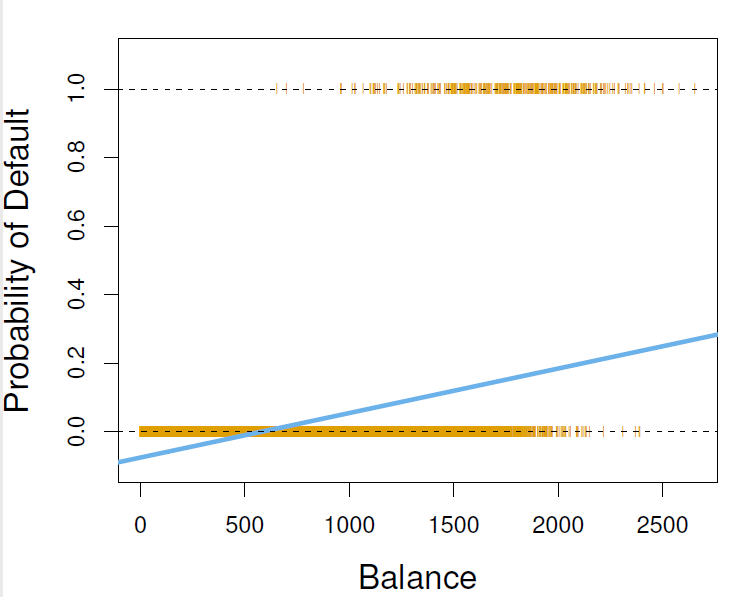
\includegraphics[scale=0.5]{../../Figures/fig_logreg.png}
	\end{figure}
\end{frame}


\begin{frame}{Logistic Function}
	We apply the so-called {\bf logistic function}
	\begin{equation*}
		p(X)= \frac{\exp(\theta_0+ \theta_1 X)}{1+ \exp(\theta_0+\theta_1 X)} 
	\end{equation*}
	After some algebraic manipulation, we can show that
	\begin{equation}
		\log \left( \frac{p(X)}{1-p(X)} \right) = \theta_0 + \theta_1 X
\label{eq:logit}	
\end{equation}
The left-hand of (\ref{eq:logit}) is called the {\bf log-odds} or {\bf logit}.

For prediction, in the logistic regression model we use $\hat{p}(X)$ as follows 

\begin{equation*}
	\hat{Y}=
	\begin{cases}
		0 & \textrm{if } \hat{p}(X)  \le 0.5 \\
		1 &  \textrm{if } \hat{p}(X) > 0.5
	\end{cases}
\end{equation*}
\end{frame}

\begin{frame}{Logistic Regression Coefficients Interpretation}
	In the normal linear regression model $\theta_1$ give the average chance in $Y$ associated with a one-unit increase in $X$.  Say for instance we have a linear model
	\begin{equation*}
		{\textrm{sales}} = {\theta}_0+ {\theta}_1 \textrm{(TV units sold)}
	\end{equation*}
	Thus, the $E(\textrm{sales})$ when the TV units sold is increased by 1 unit is ${\theta}_1$.
	
	In a logistic regression model increasing $X$ by one unit changes the log odds by $\theta_1$, or equivalently it multiplies the odds by $\exp(\theta_1)$. 
	
\end{frame}

\begin{frame}{Estimating the coefficients}
	
	Whereas we can use our training data to estimate the coefficients $\theta_0$ and $\theta_1$ using a least squares approach, this is not normally used. Instead the method of {\bf maximum likelihood} is preferred. 
	
	The likelihood function is defined by 
	\begin{equation*}
		\ell (\theta_0,\theta_1)= \prod_{i:y_i=0} p(x_i) \prod_{i':y_i'=1} (1-p(x_{i'}))
	\end{equation*}
The estimates $\hat{\theta}_0$ and $\hat{\theta}_1$  are chosen to {\it maximize} this likelihood function. 
	
\end{frame}

\begin{frame}{Multiple Logistic Regression}
	As with multi linear regression, we can expand the model to accommodate more predictors
	\begin{equation*}
		\log \left( \frac{p(X)}{1-p(X)} \right) = \theta_0 + \theta_1 X_1 + \cdots+ \theta_p X_p,
	\end{equation*} 
	
	where $X=(X_1,\ldots,X_p)$ are $p$ predictors. And the corresponding logistic function is given by
	\begin{equation*}
		p(X)= \frac{\exp(\theta_0 + \theta_1 X_1 + \cdots+ \theta_p X_p)}{1 +exp(\theta_0 + \theta_1 X_1 + \cdots+ \theta_p X_p) }
	\end{equation*}
\end{frame}

\begin{frame}{Maximal Margin Classifiers}
	A {\bf hyperplane of dimension $p$} consists of the points (vectors) in $
\mathbb{R}^p$ that satisfy the condition
\begin{equation}
	\beta_0 + \beta_1 X_1 + \cdots + \beta_p X_p=0,
	\label{eq:hyper}
\end{equation}
where $X= (X_1,\ldots, X_p)^t $ is an element of $\mathbb{R}^p$. 

The hyperplane gives us a natural separation of $\mathbb{R}^p$ into two regions

\begin{equation*}
	\begin{split}
		A^-&= \{X \in \mathbb{R}^p : \beta_0 + \beta_1 X_1 + \cdots + \beta_p X_p<0 \} \\
		A^+&= \{X \in \mathbb{R}^p : \beta_0 + \beta_1 X_1 + \cdots + \beta_p X_p >0 \}
	\end{split}		
\end{equation*}

\end{frame}

\begin{frame}{Separating Hyperplanes (Visual Idea)}
	The problem of separating by a hyperplane (line in $\mathbb{R}^2$, plane in $\mathbb{R}^3$, and hyperplane for higher dimensions)
	
		\begin{figure}[h]
		\centering
		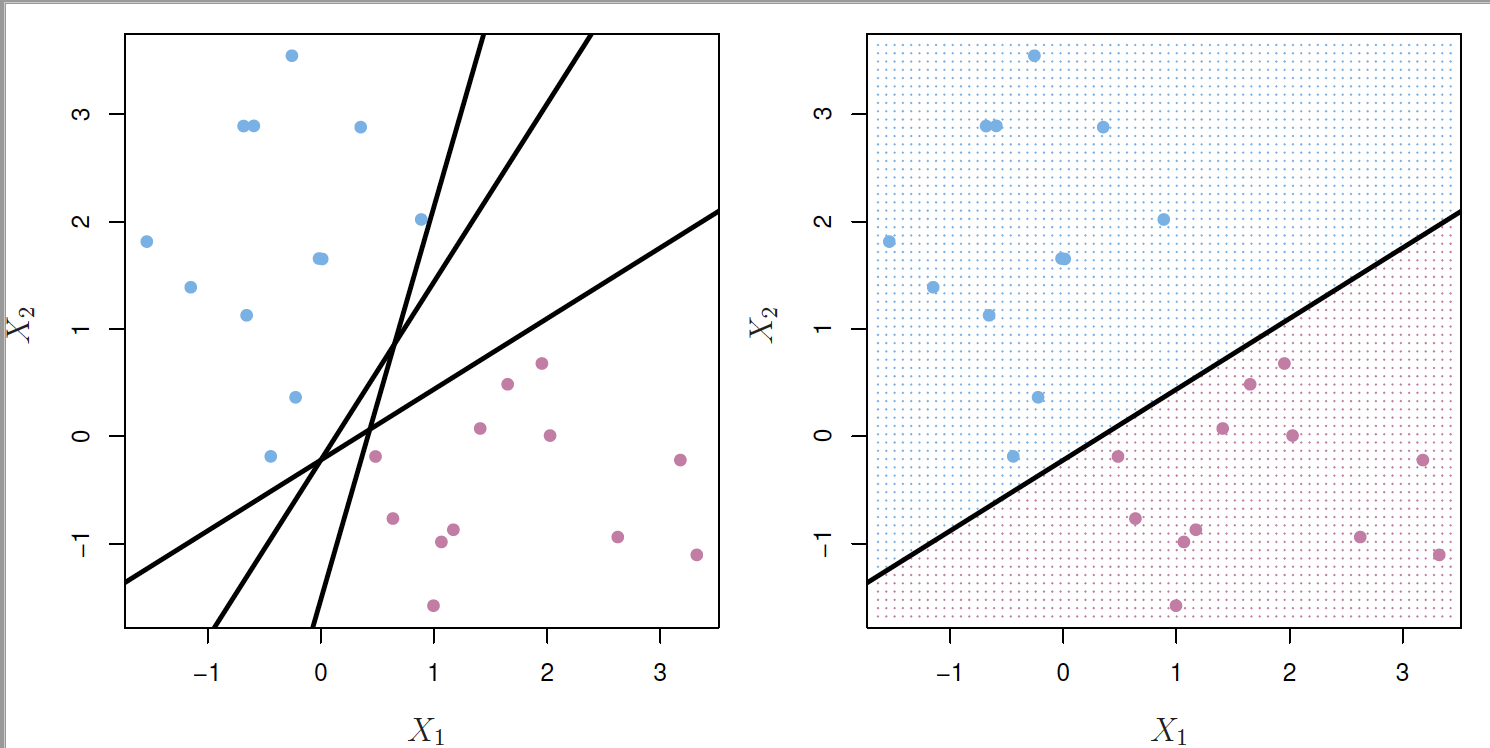
\includegraphics[scale=0.4]{../../Figures/fig_separating_line.png}
	\end{figure}
	
\end{frame}


\begin{frame}{Classification by separating hyperplanes}
	Suppose we have a $n\times p$ data matrix $\mathbf{X}$ that consists of $n$ training observations in the $p$-dimensional space
	\begin{equation*}
		x_1 = \begin{pmatrix}
			x_{11}\\ \vdots \\x_{1p} 
		\end{pmatrix}, \ldots, 
	x_n = \begin{pmatrix}
		x_{n1}\\ \vdots \\x_{np} 
	\end{pmatrix}
	\end{equation*}
and that these observations belong into either of the classes $w_1$ or $w_2$. For simplicity sake, we label the classes as a form of a  vector $Y=(y_1,\ldots,y_p)$ where $y_i \in \{-1,1\}$ for each $i$.


\end{frame}

\begin{frame}{Classification by separating hyperplanes}
	If there is a hyperplane that separates the training observations perfectly according to their labels, we call it {\bf separating hyperplane}.  Then it satisfies the conditions
	\begin{equation*}
		\begin{split}
			&\beta_0 + \beta_1 x_{i1} + \cdots + \beta_p x_{ip}<0  \quad \textrm{if } y_i = -1\\
			&\beta_0 + \beta_1 x_{i1}+ \cdots + \beta_p x_{ip}>0  \quad \textrm{if } y_i =1
		\end{split}
	\end{equation*}

Alternatively, a separating hyperplane satisfies the condition
\begin{equation*}
	y_i \left( \beta_0 + \beta_1 x_{i1} + \cdots + \beta_p x_{ip} \right)  >0  \quad \textrm{for all  } i \in \{1,\ldots,n\}
\end{equation*}
\end{frame}

\begin{frame}{Maximal Margin Classifier}
	
	Normally, if we have a separating hyperplane, there are an infinite number of alternative hyperplanes. The question is how do we select one?
	
	We will select an "optimal" plane by performing the following optimization process on the training data
	
	\begin{itemize}
		\item Compute the (perpendicular) distance from each training point to the given separating hyperplane.
		\item The minimum distance from the hyperplane defines the {\bf margin}.
		\item Select the hyperplane with the maximal margin.
	\end{itemize}
	The classification is carried out in test data by using the {\bf maximal margin classifier}. That is the sign of $f(x^*)= \beta_0 + \beta_1 x_1^* + \cdots + \beta_p x_p^*$. 
	
	The points that are equidistant from the maximal margin hyperplane are refer to as {\bf support vectors}. 
\end{frame}

\begin{frame}{Support Vectors}
	
	An important property is that the maximal margin hyperplane depends directly on only a small subset of the observations (the support vectors).
	
		\begin{figure}[h]
		\centering
		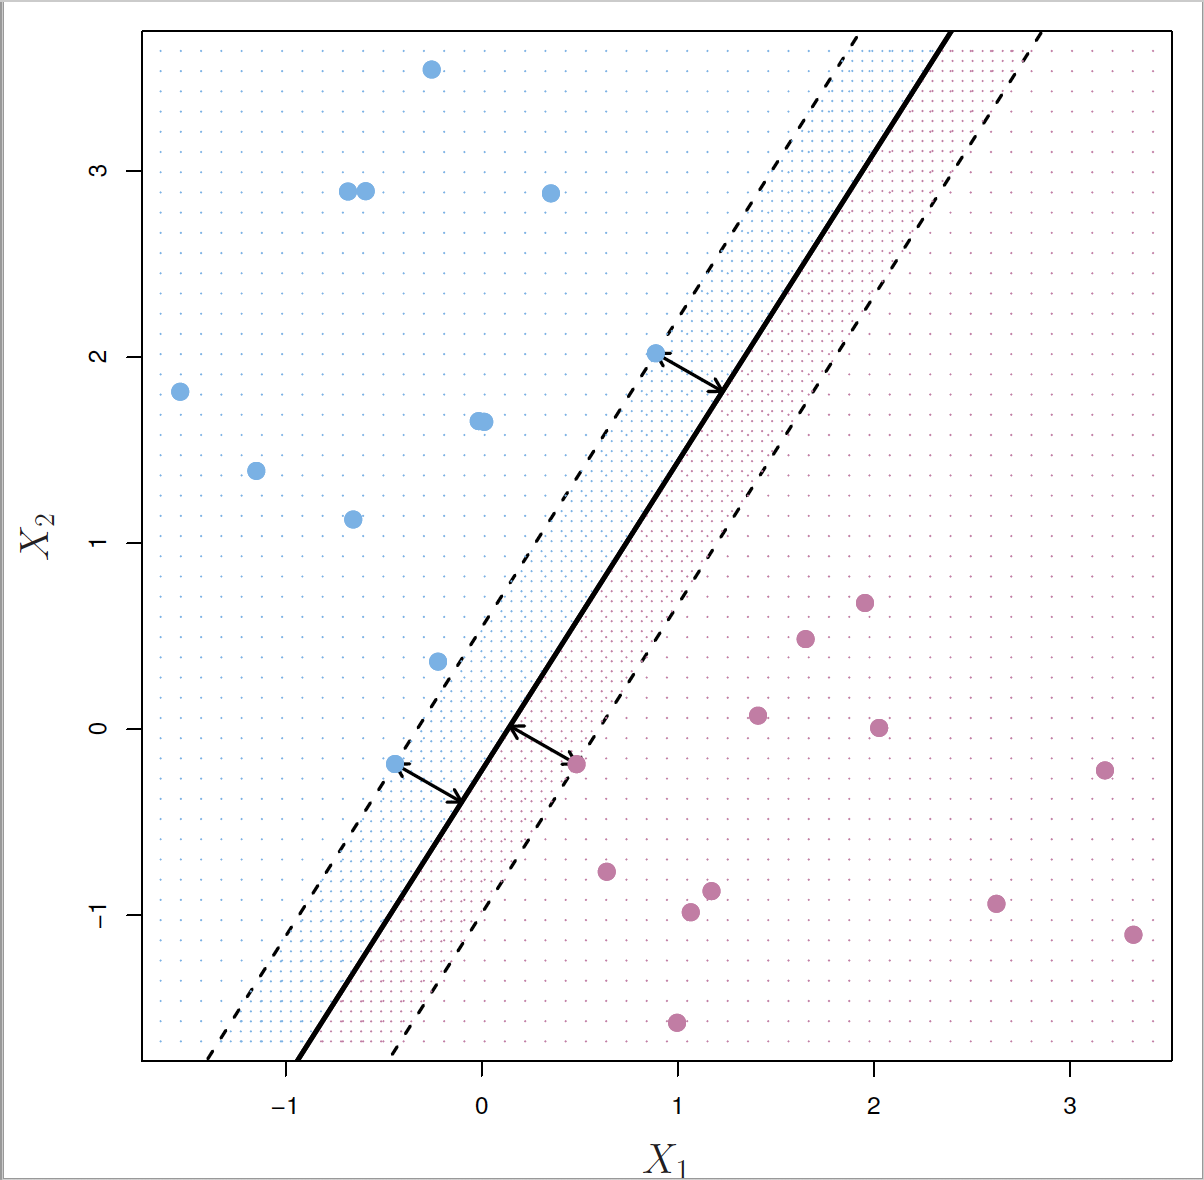
\includegraphics[scale=0.35]{../../Figures/fig_support_vectors.png}
	\end{figure}	
\end{frame}

\begin{frame}{Construction of the Maximal Margin Classifier}
	
	Finding the maximal margin hyperplane corresponds to finding a solution to the optimization problem
	
	\begin{equation*}
		\begin{split}
			&\textrm{maximize }_{\beta_0,\ldots, \beta_p} M \\
			&\textrm{subject to } \sum_{j=1}^p \beta_j^2 =1 , \\
			& y_i (\beta_0 + \beta_1 x_{i1}+ \cdots + \beta_p x_{ip} )\ge M \quad \forall i \in \{1,\ldots,n\}
		\end{split}
	\end{equation*}
where our $n$ training observations are $x_{i}$ and $Y$ is the vector with the class labels. 
\end{frame}

\begin{frame}{Non-separable Case}
	There are instances in which we cannot find the separating plane.
	
	One way to get around this problem is to introduce {\bf soft margins}, which means that we allow observations to be on the incorrect side of the margin, or even the incorrect side of the hyperplane. 
	\begin{equation*}
		\begin{split}
			&\textrm{maximize }_{\beta_0,\ldots, \beta_p,\epsilon_1,\ldots,\epsilon_n} M \\
			&\textrm{subject to } \sum_{j=1}^p \beta_j^2 =1 , \\
			& y_i (\beta_0 + \beta_1 x_{i1}+ \cdots + \beta_p x_{ip} )\ge M (1-\epsilon_i) \\
			& \epsilon_i \ge 0, \sum_{i=1}^n \epsilon_i \le C 
		\end{split}
	\end{equation*}
	where $C$ is a hyperparameter that will be tuned.
	
	 
\end{frame}
\begin{frame}{Support Vector Classifier}
The variables $\epsilon_i$ are calle {\bf slack variables} that allow individual observations to be on the wrong side of the margin or the hyperplane. More precisely, if $\epsilon_i=0$ the the $i$th observation is on the right side of the margin. If $0< \epsilon_i \le 1$, the $i$th observation is on the wrong side of the margin. If $\epsilon_i>1$ the observation $i$th is on the wrong side of the hyperplane. 

The hyperparameter $C$ limits the tolerance that we allow for the observations to be either on the wrong side of the margin or hyperplane. It controls the bias-variance trade-off. If $C$ is large, the margin is wider and we allow more violations; this amounts to fitting the data less hard and increasing bias but decreasing variance. On the other hand, if $C$ is small, we fit very tightly our model, so a low bias but high variance. 


Observation that lie directly on the margin, or on the wrong side of the margin for their class, are known as {\bf support vectors}.
\end{frame}

\begin{frame}{Variable $C$}
	
		\begin{figure}[h]
	\centering
	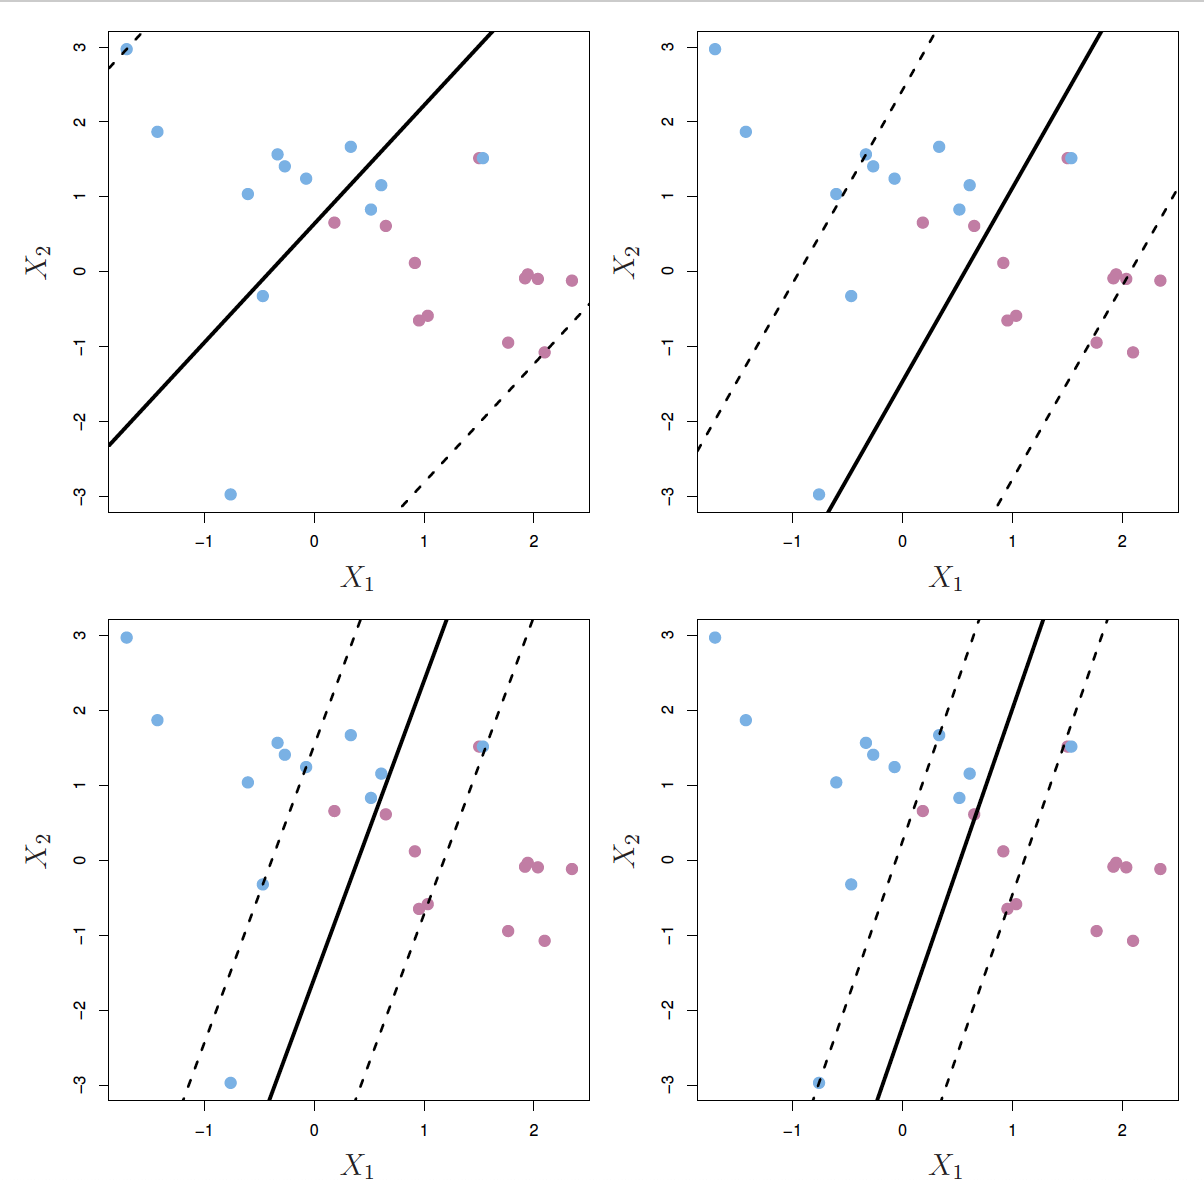
\includegraphics[scale=0.35]{../../Figures/fig_changing_c_svm.png}
\end{figure}
	
\end{frame}

\begin{frame}{Support Vector Machines}
	
	We generalize the previous problem by expanding the number of features. Say, instead of of fitting a support vector classifier using $p$ features
	\begin{equation*}
		X_1,\ldots, X_p,
	\end{equation*}
we could instead fit a support vector classifier using $2p$ features 

\begin{equation*}
	X_1,X_1^2,X_2,X_2^2,\ldots, X_p,X_p^2
\end{equation*}
In this case, the optimization process becomes
\begin{equation*}
	\begin{split}
		&\textrm{maximize }_{\beta_0,\beta_{11},\beta_{12},\ldots,\beta_{1p} \beta_{2p},\epsilon_1,\ldots,\epsilon_n} M \\
		&\textrm{subject to } y_i (\beta_0 + \sum_{j=1}^p \beta_{j1} x_{ij} + \sum_{j=1}^n \beta_{j2}x_{ij}^2)\ge M (1-\epsilon_i) \\
		&\sum_{j=1}^p \sum_{j=1}^2 \beta_{j2}x_{ij}j^2 =1 ,  \epsilon_i \ge 0, \sum_{i=1}^n \epsilon_i \le C 
	\end{split}
\end{equation*}
\end{frame}

\begin{frame}{Support Vector Machines}
	
	As we saw in the example above,  one way to extend the support vector classifier is enlarging the feature space by the so-called {\bf kernels}
	
	Instead of using the observations, we will use the {\bf inner product}  of them. The dot product is a form of an inner product
	
	\begin{equation*}
		\langle  x_i, x_{i'} \rangle = \sum_{j=1}^p x_{ij} x_{i'j}
	\end{equation*}
	In this framework, the linear support classifier can be represented as
	\begin{equation*}
		f(x) =\beta_0 + \sum_{i=1}^n \alpha_i \langle x,x_i \rangle
	\end{equation*}
Note that for the estimation of $\beta_0$ and $\alpha_i$ we need the $n \choose 2$ inner products $\langle x_i,x_{i'} \rangle$ between all pairs of training observations. However, this expression simplifies because the if $x_i$ is not a support vector $\alpha_i=0$. 
\end{frame}

\begin{frame}{Other kernels}
	
	
	We can replace the inner product with other kernels: 
	
	\begin{itemize}
		\item Polynomial kernel of degree d
		\begin{equation*}
			K(x_i,x_{i'})= (1 + \sum_{j=1}^p x_{ij}x_{i'j})^d
		\end{equation*}
	\item Radial kernel
	\begin{equation*}
K(x_i,x_{i'})= \exp \left( -\gamma \sum_{j=1}^p (x_{ij}-x_{i'j})^2 \right)
	\end{equation*}
\item Neural network
\begin{equation*}
	K(x_i,x_{i'})=\tanh (\kappa_1\langle x,x' \rangle + \kappa_2)
\end{equation*}
	\end{itemize}
\end{frame}

\begin{frame}{SVMs with different kernels}
			\begin{figure}[h]
		\centering
		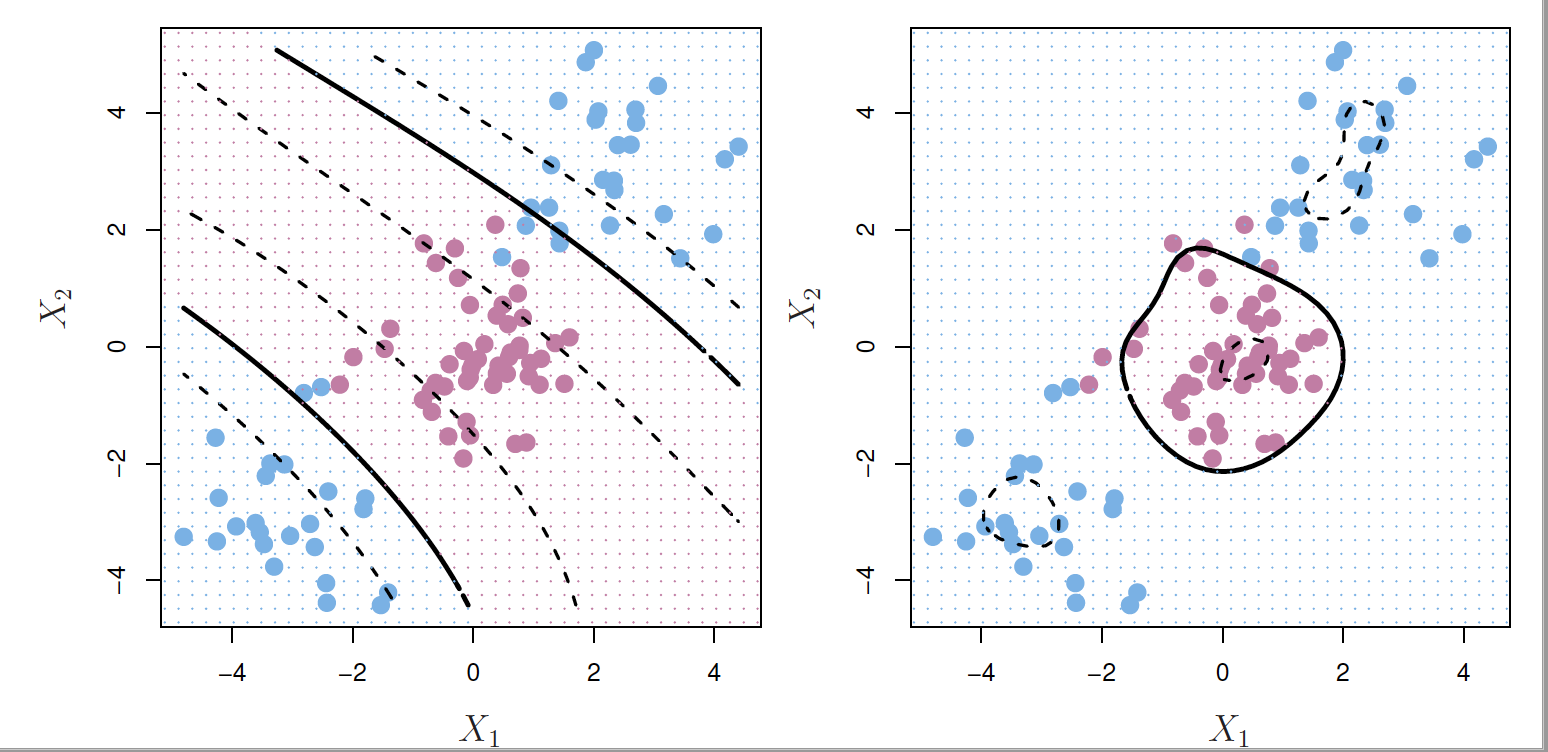
\includegraphics[scale=0.35]{../../Figures/fig_kernels_svm.png}
	\end{figure}
In the left, we have a polynomial kernel of degree 3, on the right we have a radial kernel.
\end{frame}


\begin{frame}{Rough Optimization Ideas}
	
	
	Let's start with an equivalence
		\begin{equation*}
		\begin{split}
			&\textrm{maximize }_{\beta_0,\ldots, \beta_p,\epsilon_1,\ldots,\epsilon_n} M \\
			&\textrm{subject to } \sum_{j=1}^p \beta_j^2 =1 , \\
			& y_i (\beta_0 + \beta_1 x_{i1}+ \cdots + \beta_p x_{ip} )\ge M (1-\epsilon_i) \\
			& \epsilon_i \ge 0, \sum_{i=1}^n \epsilon_i \le C 
		\end{split}
	\end{equation*}
With the following (dropping the norm constrain in $\beta$ and define $C=1/\| \beta \|$)
		\begin{equation}
		\begin{split}
			&\textrm{minimize }_{\beta_0,\ldots, \beta_p,\epsilon_1,\ldots,\epsilon_n} \| \beta \| \\
			&\textrm{subject to }  y_i (\beta_0 + \beta_1 x_{i1}+ \cdots + \beta_p x_{ip} )\ge  (1-\epsilon_i) \\
			& \epsilon_i \ge 0, \sum_{i=1}^n \epsilon_i \le \textrm{constant} 
		\end{split}
	\label{eq:optimization}
	\end{equation}
\end{frame}

\begin{frame}{Optimization Problem}
	
	The problem (\ref{eq:optimization}) is quadratic with linear inequality constrains, hence it is a convex optimization problem. We rewrite this problem as
	\begin{equation*}
		\begin{split}
	&\min_{\beta,\beta_0} \frac{1}{2}\| \beta \|^2 + \gamma \sum_{i=1}^N \epsilon_i  \\
	& \textrm{subject to } \epsilon_i \ge 0, y_i ( x_i^T \beta + \beta_0) \ge 1 -\epsilon_i \forall i
		\end{split}
	\end{equation*}
	The Lagrange (primal) function is 
	\begin{equation}
		\begin{split}
L_p=& \frac{1}{2} \|\beta\|^2 + \gamma \sum_{i=1}^N \epsilon_i -  \\
&\sum_{i=1}^{N} \alpha_i [ y_i (x_i^T \beta + \beta_0)-(1-\epsilon_i)] - \sum_{i=1}^{N} \mu_i \epsilon_i
		\end{split}
	\label{eq:lagrange}
	\end{equation}
which is minimized with respect to $\beta, \beta_0$ and $\epsilon_i$. Using calculus we take partial derivatives and make them zero.
\end{frame}

\begin{frame}{Optimization Problem}
	
	\begin{equation}
		\begin{split}
			\beta&= \sum_{i=1}^N \alpha_i y_i x_i \\
			0 &= \sum_{i=1}^N \alpha_i y_i,\\
			\alpha_i & \gamma - \mu_i \quad \forall i
		\end{split}
	\label{eq:optimization1}
	\end{equation}
as well as the positivity constrains $\alpha_i,\mu_i,\epsilon_i \ge 0$ for all $i$. If we substitute (\ref{eq:optimization1}) into (\ref{eq:lagrange}), we obtain the Lagrangian(Wolfe) dual objective function 

\begin{equation}
	L_D= \sum_{i=1}^N \alpha_i - \frac{1}{2} \sum_{i=1}^N \sum_{i'=1}^N \alpha_i \alpha_{i'} y_i y_{i'} x_i^T x_{i'},
\label{eq:lagrange2}
\end{equation}
We maximize $L_D$ subject to $0 \le \alpha_i \le \gamma$ and $\sum_{i=1}^N \alpha_i y_i=0$.
\end{frame}

\begin{frame}{What we have learned?	}
\begin{itemize}
	\item Logistic regression as a classification process
	\item Maximal margin classifier as a method for classification
	\item Support Vector classifier uses a hyperparameter to control soft limits
	\item Kernels allow us to generalize the SVM to take care of the non-linearity.
\end{itemize}
\end{frame}

\begin{frame}{References}
	Materials and some of the pictures are from \citep{James2015}, \citep{hastie01}, \citep{geron2}, and \citep{pestman}.
	\printbibliography 	
	
	I have used some of the graphs by hacking TiKz code from StakExchange, Inkscape for more aesthetic plots and other old tricks of \TeX
	
\end{frame}
\end{document}